\documentclass[10pt]{beamer}

\geometry{paperwidth=160mm,paperheight=120mm}

\usetheme[{titleformat plain}=smallcaps,
           titleformat title=smallcaps,
           titleformat subtitle=regular,
           titleformat section=smallcaps,
           titleformat frame=smallcaps,
        %    numbering=fraction,
          ]{metropolis}

\usepackage{style/main}
\usepackage[T1]{fontenc}
\usepackage[english]{babel}
\usepackage{graphicx}
\usepackage{amsmath,bm,amsfonts,amssymb,array,calc,amsthm,rotating,amscd,bbm}
\usepackage{url}
\usepackage{hyperref}
\usepackage{graphicx}
\usepackage{multicol}
\usepackage{fontawesome}
\usefonttheme[onlymath]{serif}
\usepackage[absolute,overlay]{textpos}
\setbeamercolor{background canvas}{bg=white}

\setbeamerfont{caption}{size=\scriptsize}
% \usepackage[natbib=true,backend=biber,useprefix=true]{biblatex}
% \addbibresource{references.bib}
% \setbeamercolor{bibliography item}{parent=palette primary}
% \setbeamercolor*{bibliography entry title}{parent=palette primary}

% \usetheme[progressbar=frametitle]{metropolis}
% \setbeamertemplate{frame numbering}[fraction]
% \metroset{background=dark}
% \definecolor{primary}{RGB}{245, 10, 10}
% \setbeamercolor{palette primary}{bg=white, fg=black}
% \setbeamercolor{background canvas}{parent=palette primary}
% \setbeamercolor{normal text}{fg=black}
% \setbeamercolor{progress bar}{use=palette primary, fg=primary}
% natbib=true,style=authoryear,backend=bibtex,useprefix=true
% \setbeamerfont{caption}{size=\tiny}

\usepackage[style=authoryear]{biblatex}
%%% THIS ADDS THE COMMA BETWEEN AUTHOR NAME AND YEAR
\renewcommand*{\nameyeardelim}{\addcomma\space}
\addbibresource{test.bib}


\title{Product Jacobi-Theta Boltzmann machines with score matching}
% \subtitle{Contribution to ACAT 2022}
\author{\textit{\textbf{Andrea Pasquale}}, Daniel Krefl, Stefano Carrazza, Frank Nielsen}
\date{27th October 2022, ACAT 2022, Bari}
\titlegraphic{
    \vspace*{11.5cm}
    \raisebox{20pt}[10pt][10pt]{\includegraphics[height=4cm]{../../logos/unimi_logo.pdf}}\hspace*{30pt}
    \raisebox{20pt}[10pt][10pt]{\includegraphics[height=4cm]{../../logos/tii_logo.png}}\hspace*{30pt}
    \raisebox{20pt}[10pt][10pt]{\includegraphics[height=4cm]{../../logos/infn_logo.png}}\hspace*{30pt}
    % \includegraphics[height=1.3cm]{../_logos/erc_logo1.png}

    % \vfill\vspace*{230pt}
    % \includegraphics[height=1cm]{../_logos/unimi_logo.png}\hfill
    % \includegraphics[height=1cm]{../_logos/infn_logo.png}\\
    % \vspace*{5pt}
    % {
    %     \fontsize{3pt}{3.5pt}\selectfont
    %     \begin{center}
    %         This project has received funding from the European Union's Horizon
    %         2020 research and innovation programme under grant agreement No
    %         % 740006\quad \includegraphics[height=5pt]{../_logos/eu-flag.jpg}
    %     \end{center}
    % }
}


\begin{document}

\maketitle

\section{Introduction}

\begin{frame}{Introduction}
    We started this project aiming to build a model with:
    \begin{itemize}
        \item well suited for pdf estimation and pdf sampling 
        \item built-in pdf normalization (close form expression)
        \item very flexible with a small number of parameters
    \end{itemize}
    We started from Boltzmann Machines (BM).
    \begin{figure}
        \begin{center}
            \includegraphics[scale=0.5]{figures/cauchy.pdf}
            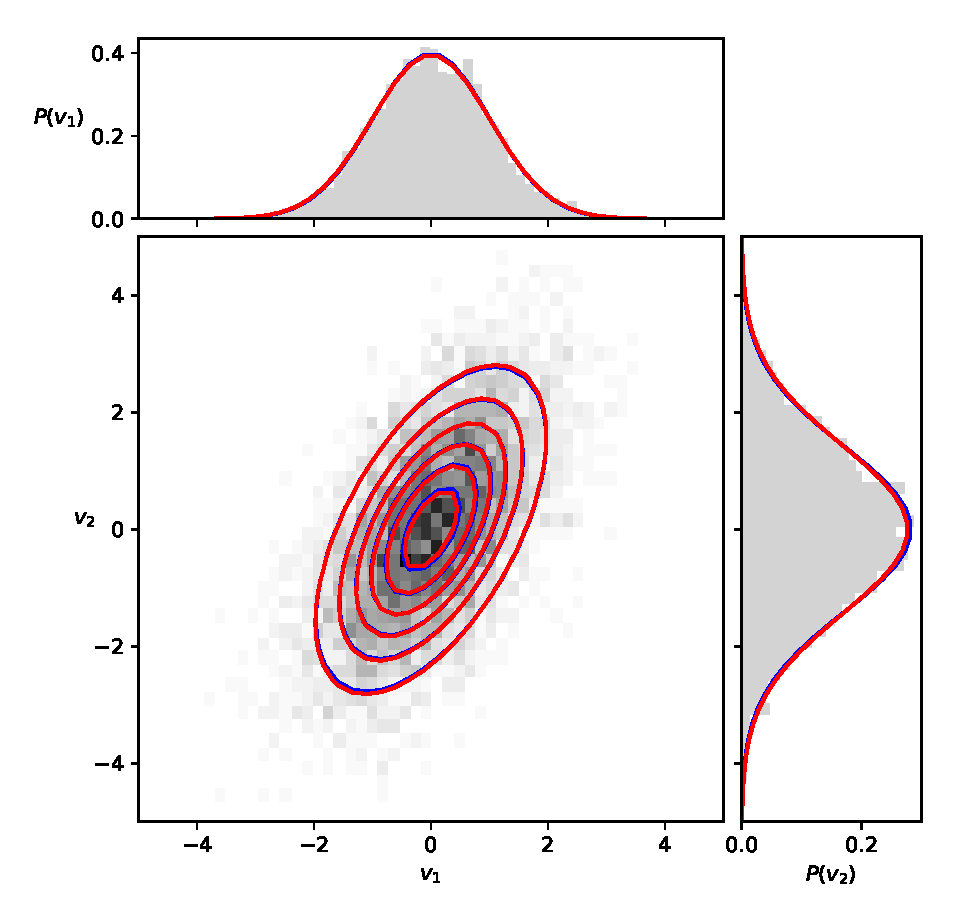
\includegraphics[scale=0.4]{figures/Gaussian2d.eps}
        \end{center}
    \end{figure}
\end{frame}
\section{Theory}

\begin{frame}{{Boltzmann Machine (BM)}}
    \begin{columns}
        \begin{column}[]{0.5 \textwidth}

            Graphical representation
            \begin{figure}
                \includegraphics[width=\textwidth]{figures/rtbm.pdf}
            \end{figure}
        \end{column}
        \begin{column}[]{0.5 \textwidth}
            Main Features:
            \begin{itemize} 
                \item Visible sector with $N_v$ nodes
                \item Hidden sector with $N_h$ nodes
                \item Binary valued states \textbf{\{0,1\}} all the nodes
                \item Connection matrices $Q$, $T$ and $W$ between the nodes
            \end{itemize}
        \end{column}
    \end{columns}
    This can be viewed as a statistical system with the following energy for a given state $(v, h)$:
    \begin{equation*}
        E(v, h) = \frac{1}{2} v^t T v + \frac{1}{2} h^t Q h + v^t W h + B_h h + B_v v
    \end{equation*}
    The probability of finding the system in the state $v$ can be computed by marginalizing $h$
\begin{equation*}
    P(v) = \sum_h \frac{e^{- E(v,h)}}{Z}
\end{equation*}  
    
    
\end{frame}





\begin{frame}{Density estimation using BM?}
    \metroset{block=fill}
    \begin{block}{Can we use BM to perform density estimation?}
        \begin{itemize}
            \pause
            \item Theoretically \textbf{yes}, since  $P(v)$ is a \textbf{parametric} density.
            \pause
            \item Practically \textbf{no} for a generic BM.
        \end{itemize}
     \end{block}
    \pause
    \emph{Density estimation is possible only using Restricted BM (RBM).}

    \begin{figure}
        \includegraphics[width= 0.7 \textwidth]{restricted.png}
    \end{figure}
    A RBM has trivial visible to visible and hidden to hidden units connections ($Q=T=0$) 
\end{frame}

\begin{frame}{A new approach to BM}
    Can we keep the inner sector couplings non-trivial, but the machine solvable?

    A possible solution is to go from binary values states to continuos/quantized values.

    If we let $v_i \in \mathbb{R}$ and $h_j \in \mathbb{R}$ we get a
    \emph{Continuous Boltzmann machine}

    \begin{equation*}
        P(v)= \frac{e^{-\frac{1}{2}v^t(T-W Q^{-1}W^t)v +B_h^t Q^{-1} W^t v  - \frac{1}{2}B^tA^{-1}B +\frac{1}{2}B^t_h Q^{-1} B_h  }  }{(2\pi )^{\frac{N_v}{2}} \sqrt{\det((T-W Q^{-1}W^t)^{-1})}  } \,,
    \end{equation*}
    which is essentially a multivariate Gaussian $\Rightarrow$ trivial model.

    If instead we let $v_i \in \mathbb{R}$ and $h_j \in \mathbb{Z}$ we get the following
    \begin{equation*}
        P(v) = \sqrt{\frac{\det T}{(2\pi)^{N_v}}} e^{- \frac{1}{2} v^t T v - B_v^t v - B_v^t T^{-1} B_v}
            \frac{\tilde{\theta}(B^t_h+v^t W \vert Q)}
            {\tilde{\theta}(B^t_h-B_v^t T^{-1} W \vert Q - W^t T^{-1} W)} \ .
    \end{equation*}
    \begin{center}
        \textbf{non-trivial closed form solution under mild constraints!}
    \end{center}

\end{frame}

\begin{frame}{Riemann-Theta BM \hfill \small [\cite{2020}]}
    Lets take a closer look at the probability density
    \begin{equation*}
        P(v) = \sqrt{\frac{\det T}{(2\pi)^{N_v}}} e^{- \frac{1}{2} v^t T v - B_v^t v - B_v^t T^{-1} B_v}
            \frac{\tilde{\theta}(B^t_h+v^t W \vert Q)}
            {\tilde{\theta}(B^t_h-B_v^t T^{-1} W \vert Q - W^t T^{-1} W)} \ .
    \end{equation*}
    
    Multivariate gaussian modulated by the functions $\theta$ which are known as
    Riemann-Theta functions:
    \begin{equation*}
        \theta ( z, \Omega) :=
        \sum_{n \in \mathbb{Z}^N} e^{2 \pi i \big( \frac{1}{2}n^t \Omega n + n^t z \big)} \ .
    \end{equation*}
    Therefore we called this model Riemann-Theta BM or RTBM.
    % \textbf{Key properties}: quasi-periodicity, modular invariance, solution to physics related problem.
    \begin{figure}
        \begin{center}
          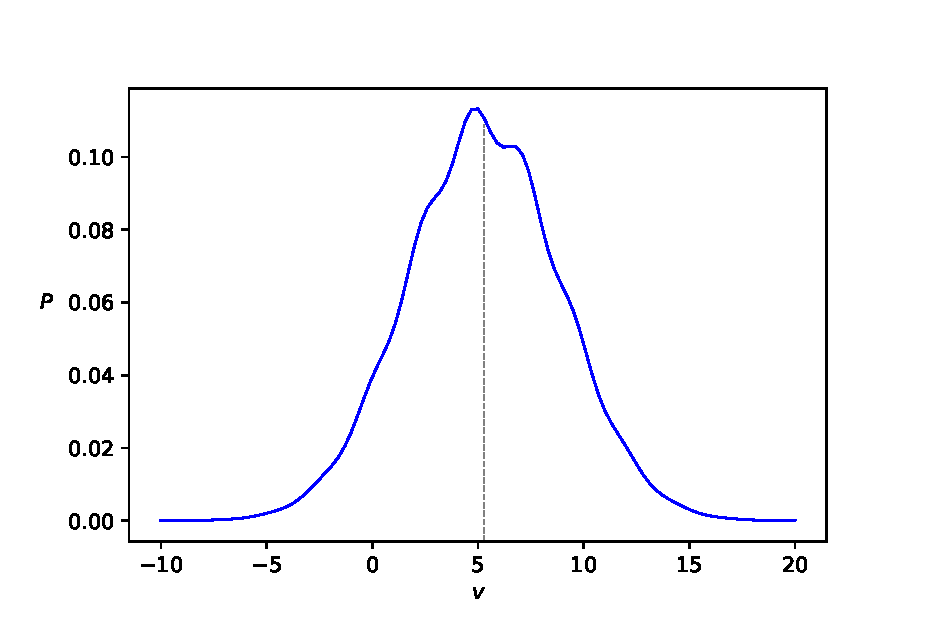
\includegraphics[scale=0.25]{figures/PvPhaseI-1}
          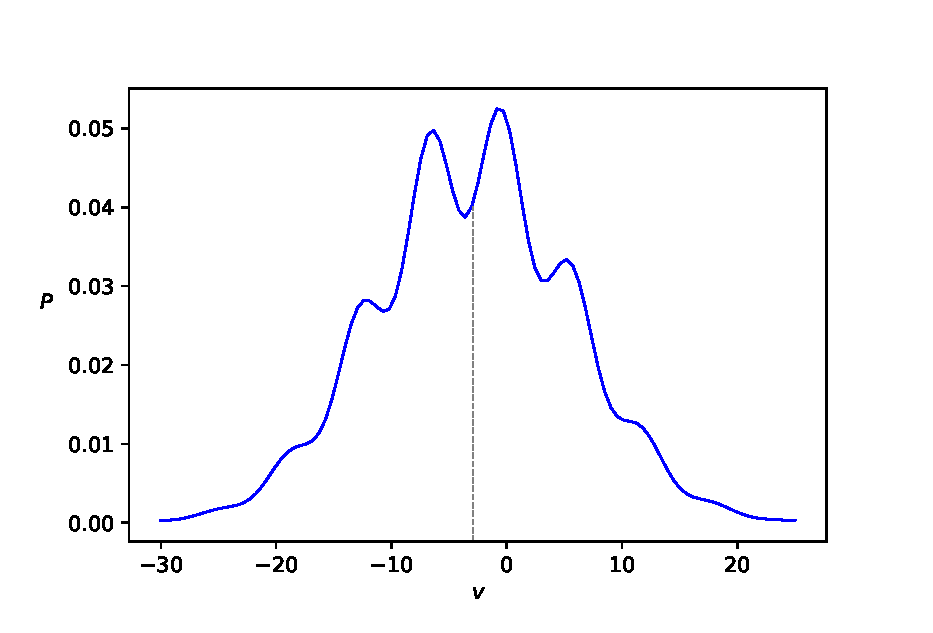
\includegraphics[scale=0.25]{figures/PvPhaseI-2}
          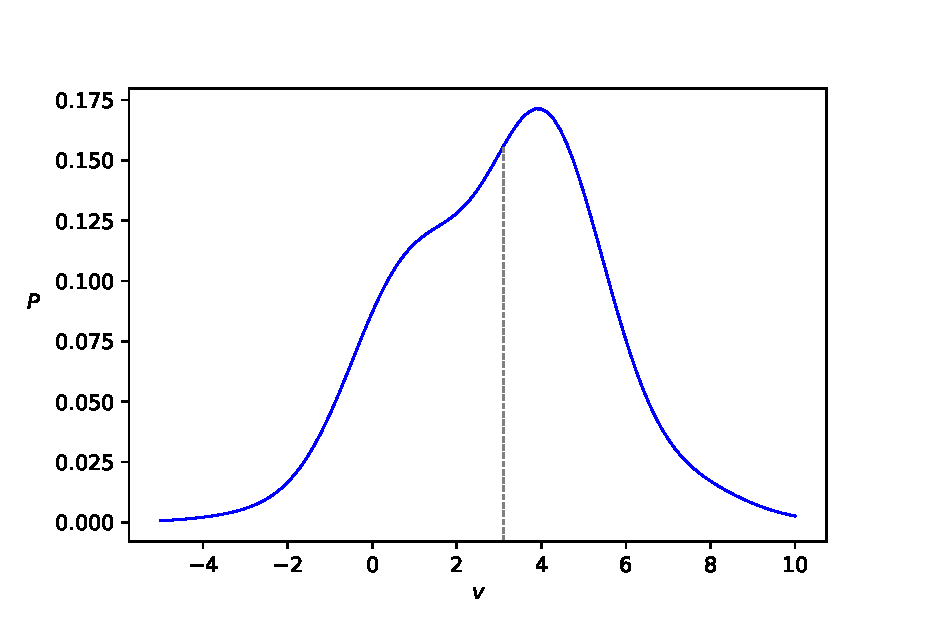
\includegraphics[scale=0.25]{figures/PvPhaseI-3}
          \includegraphics[scale=0.25]{figures/PvPhaseII-1}
          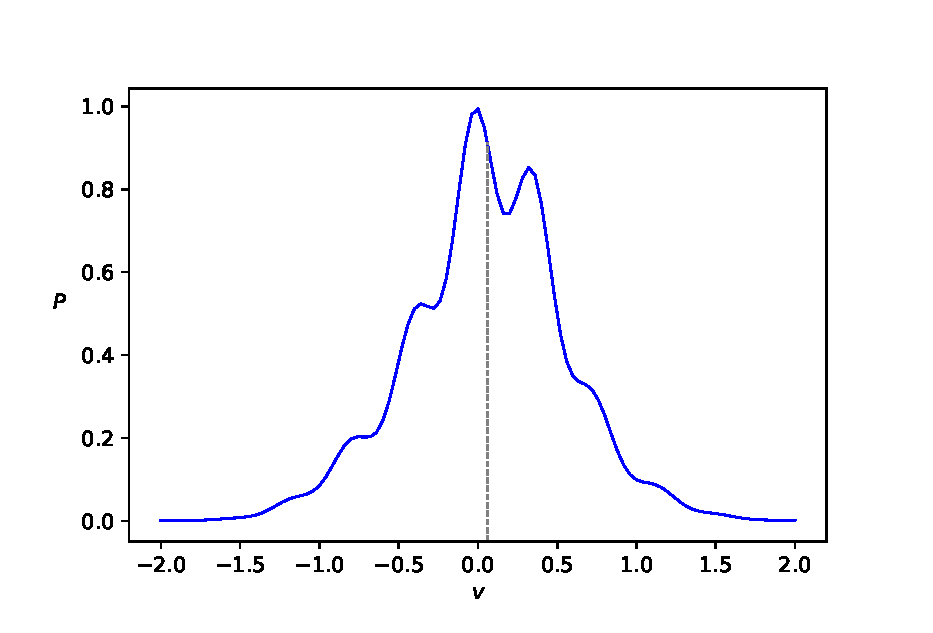
\includegraphics[scale=0.25]{figures/PvPhaseII-2}
          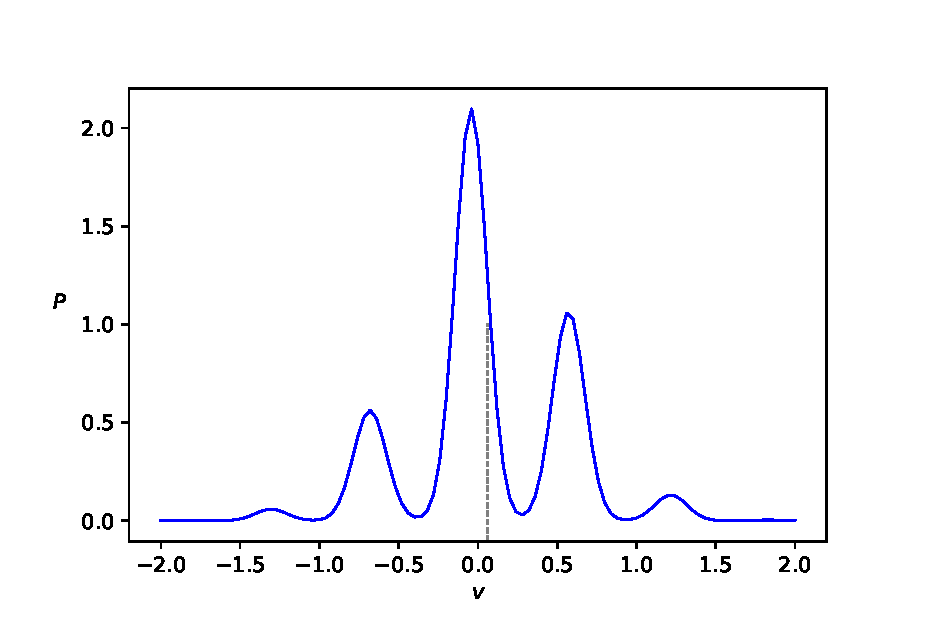
\includegraphics[scale=0.25]{figures/PvPhaseII-3} 
        %\caption{Plots of $P(v)$ for one-dimensional $v$ and various choices of parameters $B_v,B_h,W,T,Q$. Top row: Phase I. Bottom row: Phase II. The first examples in both phases are with one-dimensional Q, while the remaining plots are for $Q$ of size $2\times 2$. The gray dashed lines mark the means of the distributions.}
          \label{PvPlots}
        
        \end{center}
        \caption{ A few examples of $P(v)$ for different parameters}
        \end{figure}
        % \begin{center}
        %    .
        % \end{center}
\end{frame}


% \begin{frame}{Riemann-Theta Boltzmann Machin}
%     We can obtain a non-trivial model if we change the domain from binary values states to continuous/quantized values.
%     If we consider $v \in \mathbb{R}^{N_v}$ and $h \in \mathbb{Z}^{N_h}$, under mild constraints
%     on the connection matrices we can compute $P(v)$ in a closed form:
%     \begin{equation*}
%         P(v) = \sqrt{\frac{\det T}{(2\pi)^{N_v}}} e^{- \frac{1}{2} v^t T v - B_v^t v - B_v^t T^{-1} B_v}
%             \frac{\tilde{\theta}(B^t_h+v^t W \vert Q)}
%             {\tilde{\theta}(B^t_h-B_v^t T^{-1} W \vert Q - W^t T^{-1} W)} \ .
%     \end{equation*}
%     which corresponds to a multi-variate gaussian moldulated by the functions $\tilde{\theta}$, which
%     are known as \textbf{Riemann-Theta (RT)} functions.
%     \newline
%     We called this model the \textbf{Riemann-Theta Boltzmann Machine (RTBM)}. 

%     \begin{figure}
%         \begin{center}
%           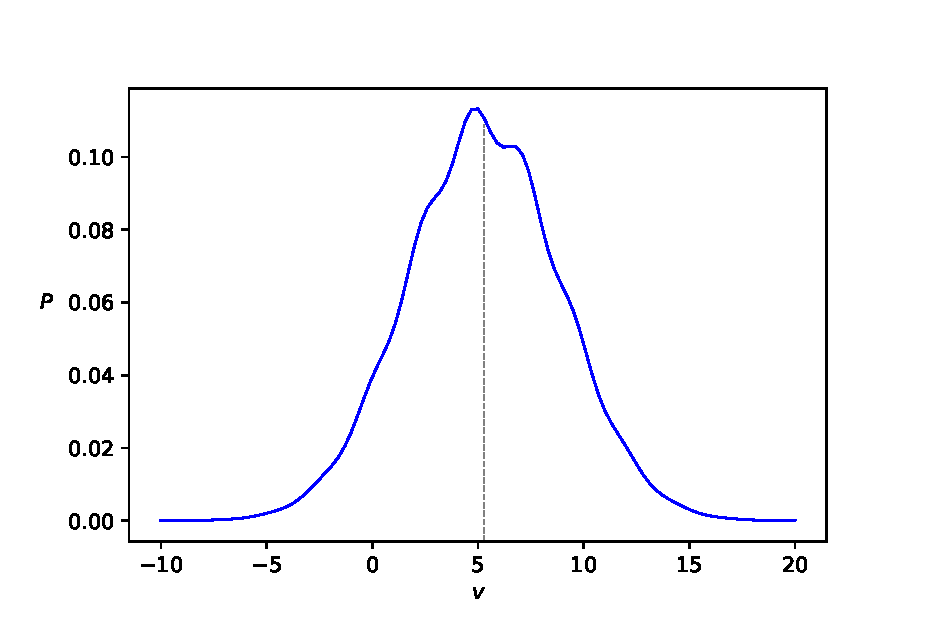
\includegraphics[scale=0.25]{figures/PvPhaseI-1}
%           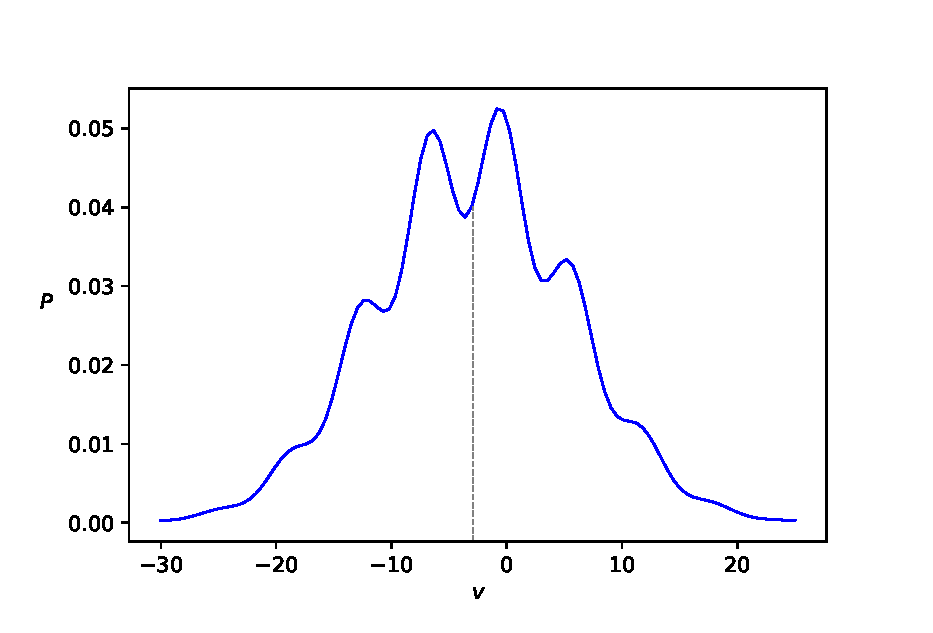
\includegraphics[scale=0.25]{figures/PvPhaseI-2}
%           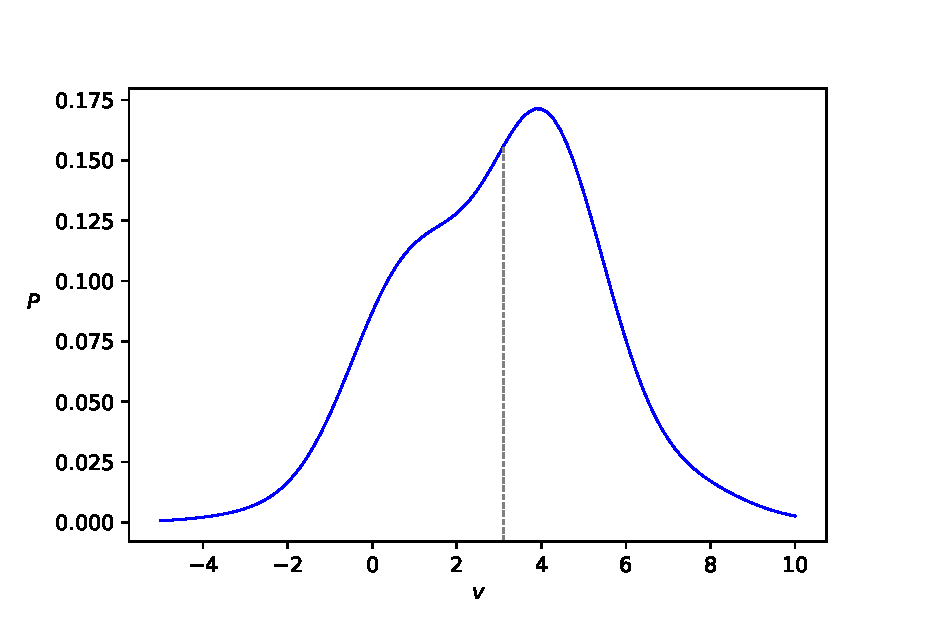
\includegraphics[scale=0.25]{figures/PvPhaseI-3}
%           \includegraphics[scale=0.25]{figures/PvPhaseII-1}
%           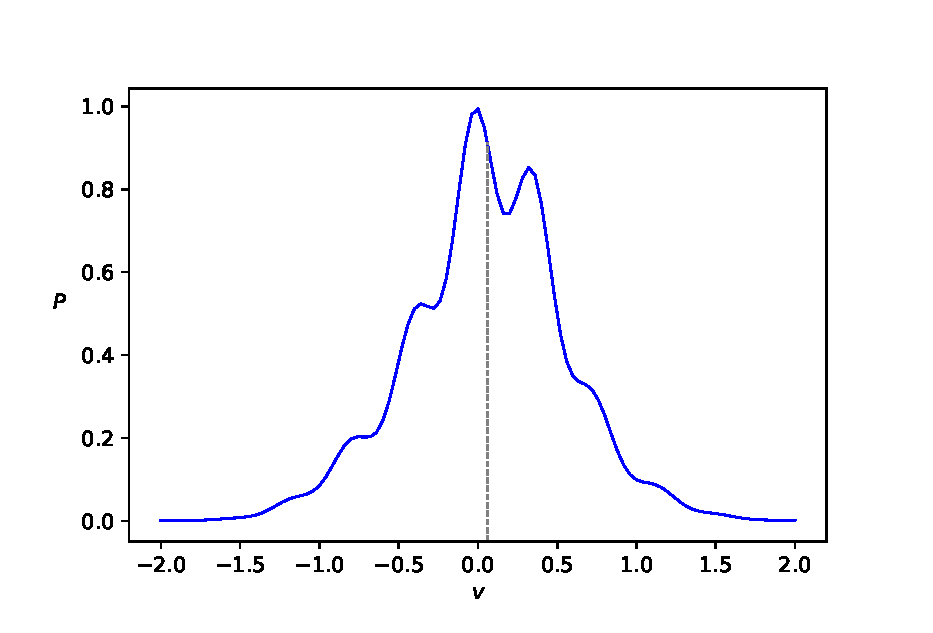
\includegraphics[scale=0.25]{figures/PvPhaseII-2}
%           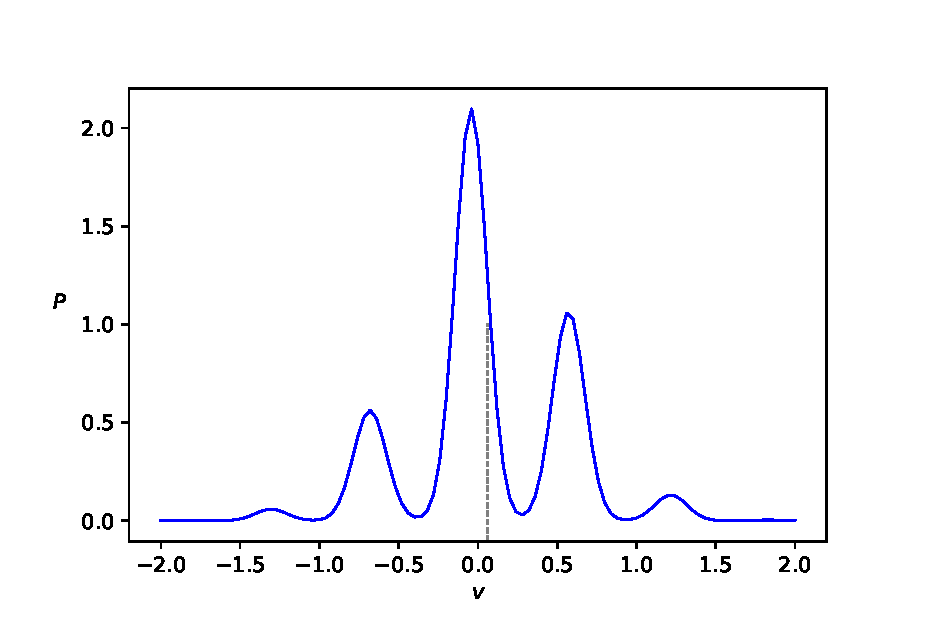
\includegraphics[scale=0.25]{figures/PvPhaseII-3} 
%         %\caption{Plots of $P(v)$ for one-dimensional $v$ and various choices of parameters $B_v,B_h,W,T,Q$. Top row: Phase I. Bottom row: Phase II. The first examples in both phases are with one-dimensional Q, while the remaining plots are for $Q$ of size $2\times 2$. The gray dashed lines mark the means of the distributions.}
%           \label{PvPlots}
        
%         \end{center}
%         \end{figure}
%         \begin{center}
%             A few examples of $P(v)$ for different parameters.
%         \end{center}
       
% \end{frame}

\section{Properties of RTBMs}

\begin{frame}{Learning \hfill \small [\cite{2020}]}
    With a RTBM we can perform density estimation to learn the parameters via
    maximum likelihood. That is, for $N$ samples $x_i$ from an unknown
    probability density we take the cost function
   
    \begin{equation*}
        \mathcal{C}  = - \sum_{i=1}^N \log  P(x_i)
        \end{equation*}

    and we solve the optimization problem:
    \begin{equation*}
            \argmin_{Q,T,W,B_h,B_v} \mathcal{C}
        \end{equation*} 

        \metroset{block=fill}
        \begin{block}{Gradient based techniques}
        Since $P(v)$ is fully analytical we can solve the optimization 
        problem using gradient or non-gradient based techniques\footnote{In this work
        we are using the CMA-ES optimizer.}.
        \end{block}
    % 
    % where $\mathcal{C}$ is an arbitrary cost function. 

    % In the case of Maximum Likelihood Estimation (MLE) we get:
    % \begin{equation*}
    %     \argmin_{Q,T,W,B_h,B_v} - \sum_{i=1}^N \log  P(x_i) = \argmax_{Q,T,W,B_h,B_v} \sum_{i=1}^N \log P(x_i)
    % \end{equation*} 
    % Since we have an analytical expression for $P(v)$ we have the possibility to use both
    % gradient or non-gradient based techniques.


\end{frame}

\begin{frame}{Examples \hfill \small [\cite{2020}]}
    \begin{figure}[t!]
        \begin{center}
        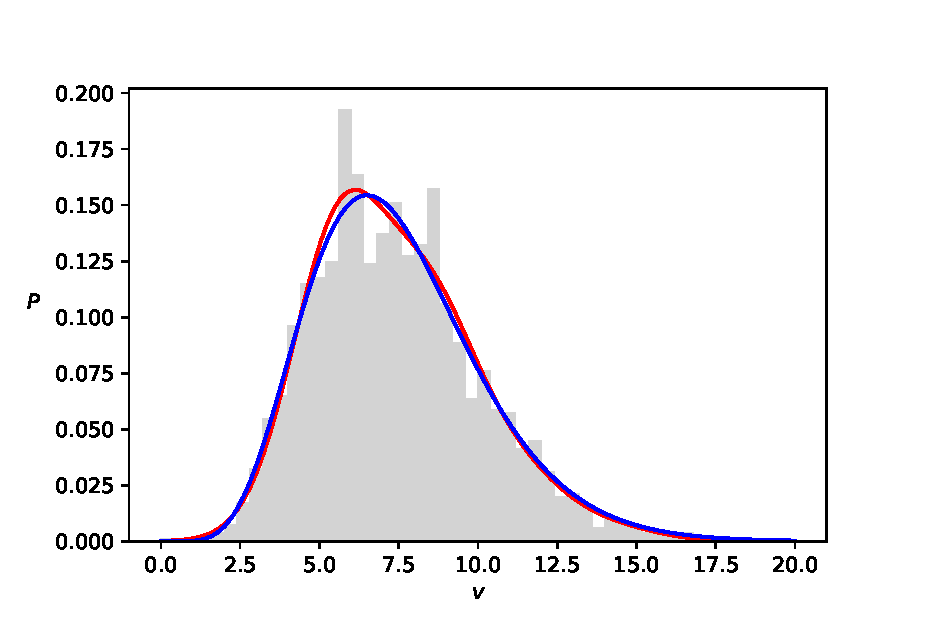
\includegraphics[scale=0.30]{figures/GammaDist}
        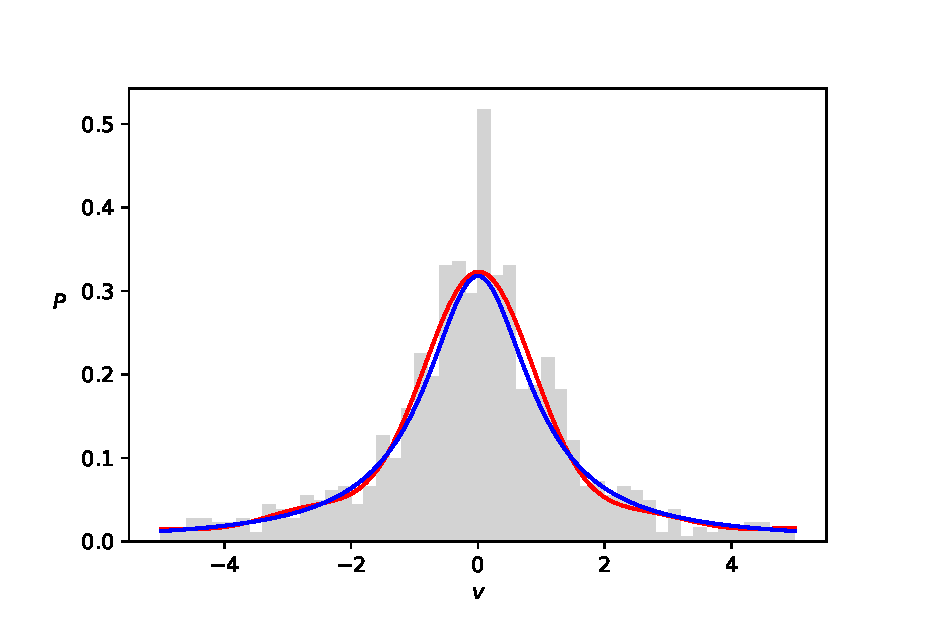
\includegraphics[scale=0.30]{figures/CauchyDist}
        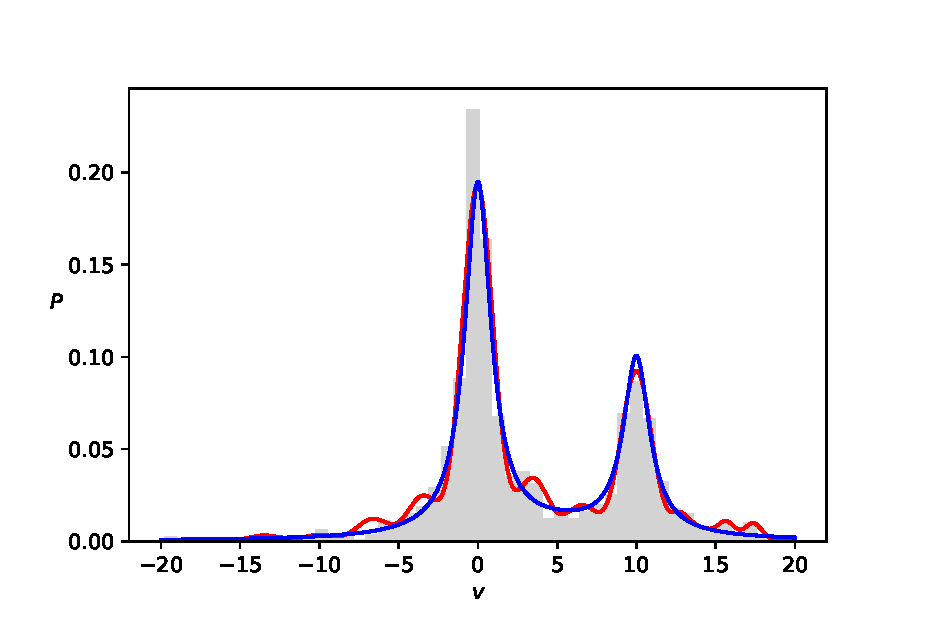
\includegraphics[scale=0.30]{figures/CauchyMix}
        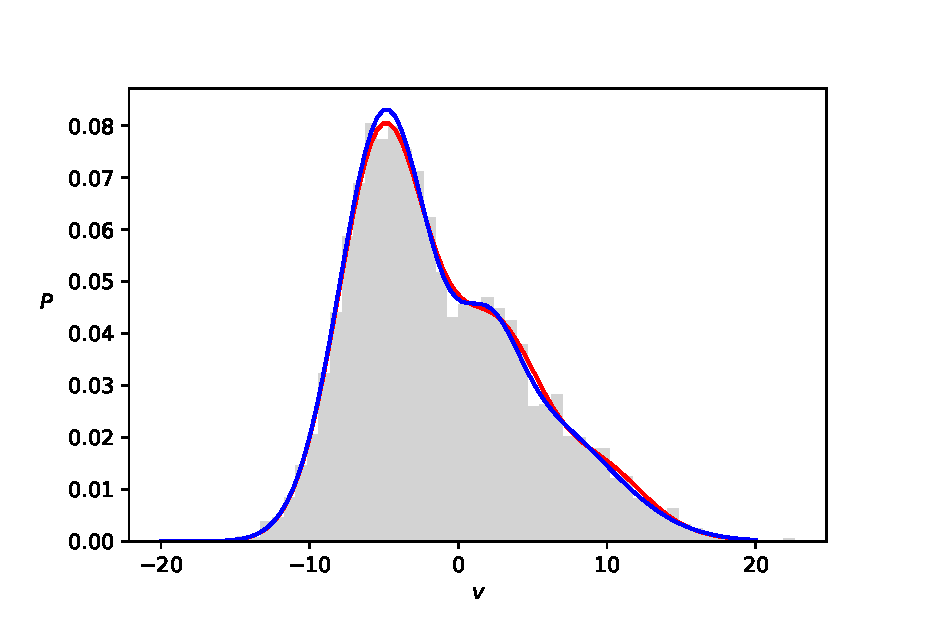
\includegraphics[scale=0.30]{figures/Gaussians}    
        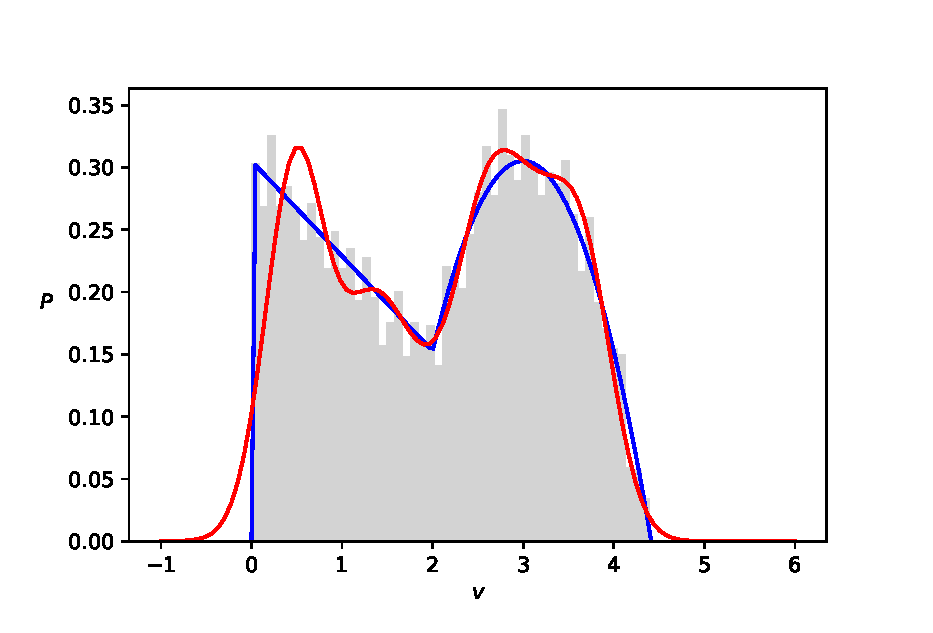
\includegraphics[scale=0.30]{figures/Likas2}  
        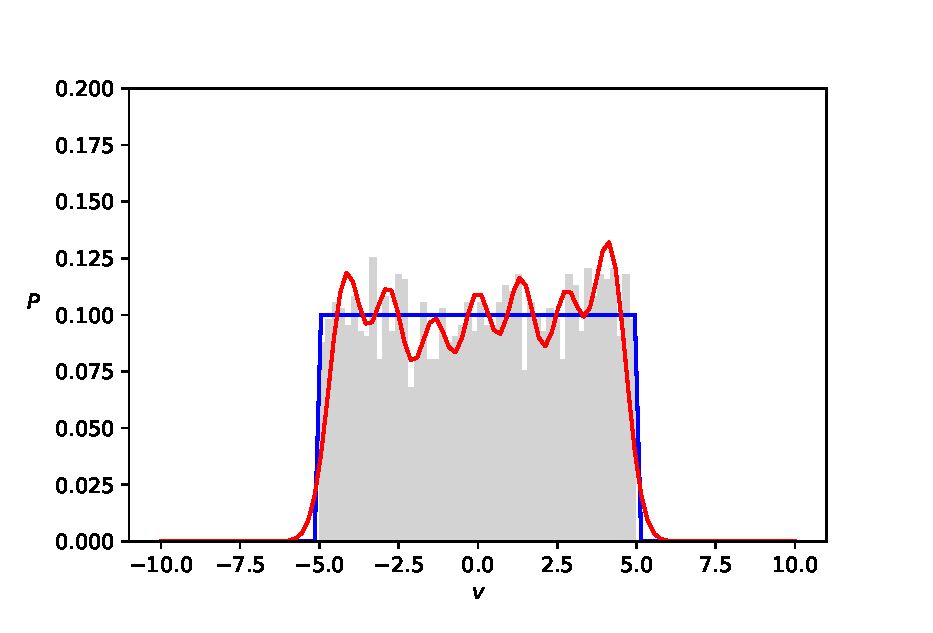
\includegraphics[scale=0.30]{figures/Likas1}

        %\caption{\tiny Top left: Gamma distribution fitted by a single RTBM with $N_{h}=2$.  Top middle: Cauchy distribution fit via a single RTBM with $N_{h}=3$. Top right: Fit of Cauchy distribution mixture via a layer of two RTBMs with $N_{h}=3$. Bottom left: Gaussian mixture fit by a single RTBM with $N_{h}=3$. Bottom middle: Custom mixture model fit using a single RTBM with $N_{h}=4$. Bottom right: Uniform distribution fit via a single RTBM with $N_h=3$. In all figures the blue line corresponds to the underlying true distribution, while the red line is the fit. The histograms show the samples the models are trained on.}
        % \label{CauchyDistFig}
        \end{center}
      \end{figure}
      \vspace{-0.5cm}
      \begin{columns}
        \begin{column}[]{0.7 \textwidth}
            \begin{figure}
                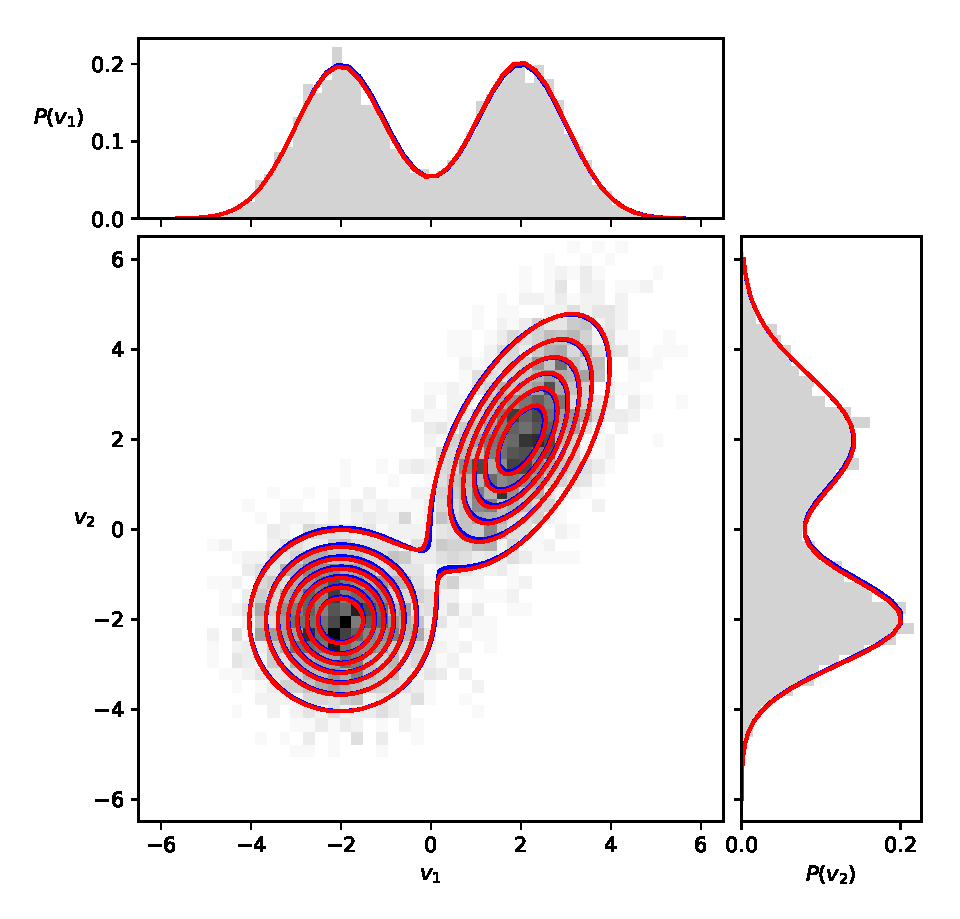
\includegraphics[scale=0.30]{figures/TwoGaussians2d.eps}    
                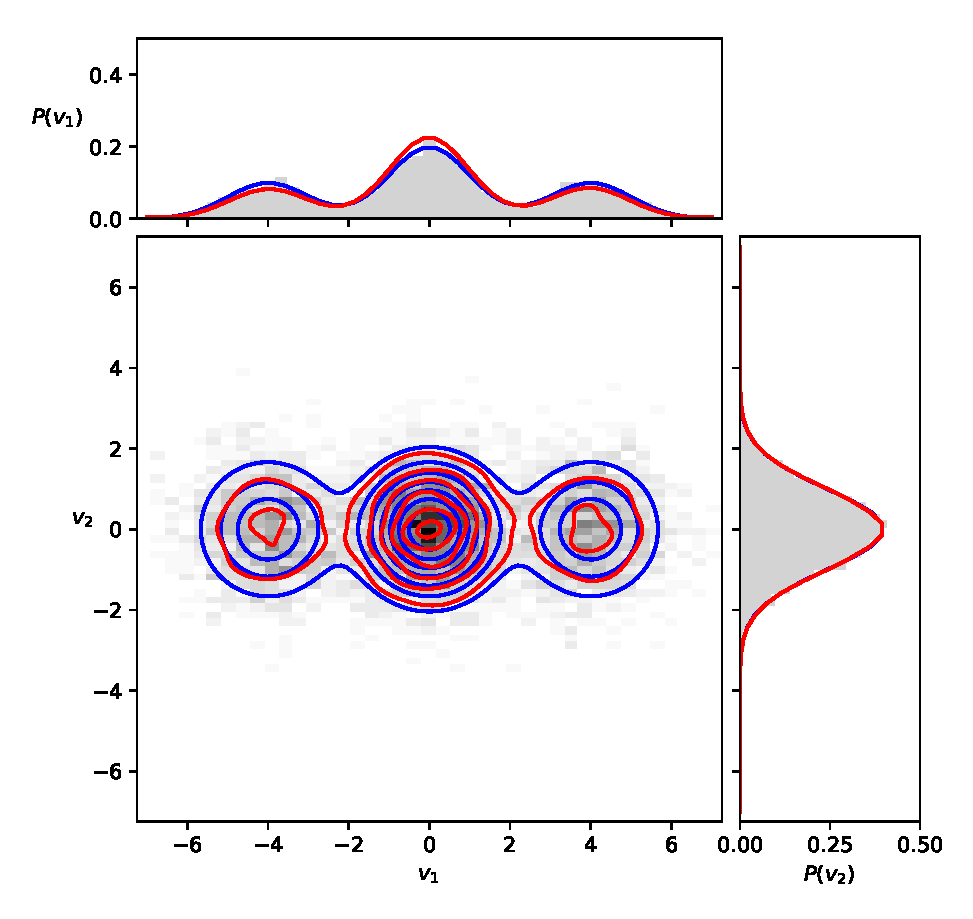
\includegraphics[scale=0.30]{figures/ThreeGaussians2d.eps} 
            \end{figure}
        \end{column}
        \begin{column}{0.3 \textwidth}
            \begin{itemize}
                \item Blue line: real distribution
                \item Red line: RTBM
                \item Histogram: sample from real distribution
            \end{itemize}
            
        \end{column}
      \end{columns}

       


Blue line: true distribution
Red Line: RTBM 
\end{frame}


\begin{frame}{Properties of RTBM \hfill \small [\cite{Carrazza:2018nmd}]}
    Over the last years we discoverd that the RTBM possesses a lot of nice properties.
    \vspace{1cm}
    \begin{columns}

        \begin{column}{0.5 \textwidth}
            \centering
            \vspace{-0.5 cm}

            \textbf{Sampling}

            \includegraphics[scale=0.40]{figures/ThreeGaussians2d-eps-converted-to.pdf}

            We can easily extract samples from $P(v)$ using numerical
            evaluation of $\theta$ functions
        \end{column}

        \begin{column}{0.5 \textwidth}
            \centering

            \textbf{Affine transformations}

            \includegraphics[scale=0.40]{figures/rotation2d.pdf}

            $P(v)$ stays in the same distribution under affine
            transformations
            $$
            \mathbf w = A \mathbf v+b\,, \quad \mathbf w \sim P_{A,b}(v)\,,
            $$
        \end{column}

        % \begin{column}{0.3 \textwidth}
        %     \textbf{Conditional probabilities}
        % \end{column}

    
    \end{columns}

\end{frame}



% \begin{frame}{Affine transformation example}
    
%     We can use this property to improve the training:
%       \begin{enumerate}
%         \item Perform affine transformation $M$ from domain $D_1$ to $D_2$.
%         \item Train the model on $D_2$ (easier)
%         \item Perform inverse affine transformation $M^{-1}$ to transform the model back to $D_1$ already trained.
%       \end{enumerate}
% \end{frame}

\section{Limitations}

\begin{frame}{Limitations}
    Despite the promising results there is one major issue: 
    \begin{center}
        \textbf{The learning process can become slow for ($N_h > 5$).} 
    \end{center}
    It is not possible to use RTBMs for:

    \begin{multicols*}{2}
        \begin{itemize}
            \item Complicated low-dimensional models
            \item High dimensional models ($N_h \geq N_v$)
        \end{itemize}
        
    \end{multicols*}
    
    \begin{center}
        \textbf{Why this happens?}
       
    \end{center}

    The computation of $\theta$ and its derivatives is a bottleneck for increasing value of $N_h$
    \footnote{The computational times increase exponentially due to the computation of
    the exponential of a $N_h \times N_h$ matrix required by the $\theta$ function.}.
    \begin{equation*}
        \theta ( z, \Omega) :=
        \sum_{n \in \mathbb{Z}^N} e^{2 \pi i \big( \frac{1}{2}n^t \Omega n + n^t z \big)} \ .
    \end{equation*}
    


\end{frame}

\section{Improving the RTBM}


\begin{frame}{Factorizability \hfill \small [\cite{new} in preparation]}
    To speed up the calculation we can exploit the following property of the $\theta$ function:
    % The RT function has an interesting property that can become useful when dealing with large matrices.
    % Lets consider the following RT function $\theta(z, \Omega)$, if we assume that $\Omega$ 
    % is diagonal the RT can be factorized as follows:
    \metroset{block=fill}
    \begin{block}{Factorizability}
        Under the assumption that $\Omega$ is a complex \textbf{diagonal} $N \times N$
        matrix, whose imaginary part is positive definite, the Riemann-Theta function
        $\theta(z, \Omega)$ factorizes
        \begin{equation}
            \label{eq:theta}
            \theta(z, \Omega) = \prod_{i=1}^N \theta(z_i, \Omega_{ii})
        \end{equation}
        \end{block}

    \vspace{-1.3    cm}
    \begin{columns}
        \begin{column}{0.7 \textwidth}
            \vspace{1cm}

            \begin{figure}
                \begin{center}
                    \includegraphics[scale=0.4]{figures/factorized.png}
                \end{center}
                \vspace{-0.8cm}

                \caption{Average time to compute the RT using \cite{deconinck2002computing}}
            \end{figure}

        \end{column}
        \begin{column}{0.5\textwidth}

            \begin{itemize}
                \item Important speed-up

                as we increase $N$

                \item Computational times
                 
                almost costant 
     
            \end{itemize}
           
        \end{column}
    \end{columns}
    

    
\end{frame}
\begin{frame}{Factorizability  \hfill \small [\cite{new} in preparation]}
    \emph{Can we exploit the previous property directly on $P(v)$?}
    \begin{equation*}
        P(v) = \sqrt{\frac{\det T}{(2\pi)^{N_v}}} e^{- \frac{1}{2} v^t T v - B_v^t - B_v^t T^{-1} B_v}
            \frac{ \tikz[baseline, remember picture]{
                \node[anchor= base] (e1) {\fcolorbox{red}{white}{$\tilde{\theta}(B^t_h+v^t W \vert Q)$}};
            }}
            {\tikz[baseline, remember picture]{
                \node[anchor= base] (e1) {\fcolorbox{blue}{white}{$\tilde{\theta}(B^t_h-B_v^t T^{-1} W \vert Q - W^t T^{-1} W)$}};
            }} \ .
    \end{equation*}

    % \begin{textblock}{4}(12,6)%
    %     \begin{scriptsize}
    %     \tikz[remember picture]{ \node (b1) {Q diagonal};}
    %     \end{scriptsize}%
    % \end{textblock}

    % \begin{tikzpicture}[remember picture, overlay]
    %     \draw [->] (b1.south) -- (e1);
    % \end{tikzpicture}
    We have to compute two $\theta$ function:
    \begin{itemize}
        \item $\tikz[baseline, remember picture]{
            \node[anchor= base] (e1) {\fcolorbox{red}{white}{$\tilde{\theta}(B^t_h+v^t W \vert Q)$}};
        }$ can we take $Q$ diagonal? \textbf{Yes}
        \item $\tikz[baseline, remember picture]{
            \node[anchor= base] (e1) {\fcolorbox{blue}{white}{$\tilde{\theta}(B^t_h-B_v^t T^{-1} W \vert Q - W^t T^{-1} W)$}};
        }$ $ Q - W^t T^{-1} W$ diagonal? \textbf{\emph{not feasible}}
    \end{itemize}
    
    
    \textbf{Obsv:} the second term is a normalization term.

    \textbf{Idea}: Can we select a specific cost function to avoid computing that term?

\end{frame}

\begin{frame}{Score Matching \hfill \small [\cite{lyu2012interpretation}]}
    A particular parameter learning methodology that can address this issue is \emph{Score Matching}, which is 
    based on the Fisher divergence.
        \begin{equation*}
            D_F(p\lvert \lvert q_\xi) = \int p(x) \Bigg\vert 
            \frac{\nabla_{x} \ p(x)}{p(x)} -
            \frac{\nabla_{x} \ q(x,\xi)}{q(x,\xi)}  \Bigg\vert^2 d x \ , 
        \end{equation*}
    which is slightly different from the Kullback-Leiber divergence:
    \begin{equation*}
        D_{KL}(p\lvert \lvert q_\xi) = \int
            p(x) \log{\frac{p(x)}{q(x,\xi)}} d x \ , 
    \end{equation*}
    
We will show in the next slide that the normalization terms cancel out since

$$ D_F  \propto \frac{d^{(i)}}{dx^{(i)}} \log q(x, \xi)$$


Therefore if we start by assuming that $Q$ is diagonal the learning process will involve
only the computation of 1d $\theta$ functions!
\end{frame}

\begin{frame}{Score Matching \hfill \small [\cite{new} in preparation]}
    We can simplify the expression for $D_F$ under the assumption that our model $q(x, \theta)$ is sufficiently regular,
    which is the case of the RTBM.
    \begin{equation*}
        \begin{split}
        D_F(p\lvert \lvert q_\theta) &=  \int p(x) \bigg(
            \big\vert \nabla_{x} \log{q(x,\theta)} \big\vert^2 +
            2 \Delta_{x} \log{q(x,\theta)}
            \bigg) + \text{const}  \\
            &\approx 
            \tikz[baseline, remember picture]{
                \node[anchor= base] (e1) {\fcolorbox{green}{white}{$\sum_{i=1}^N \Bigg \vert 
                \nabla_{v_i} \log{q(v_i, \theta)} \Bigg \vert^2
                + 2 \Delta_{v_i} \log{q(v_i, \theta)}$}};
            }
            + \text{const}\,. \\
            &\approx \mathcal{C}_F
        \end{split} 
    \end{equation*}

    We call $\mathcal{C}_F$ Fisher cost function and it is particularly useful
    for \textbf{non-normalizable} models.

    % \begin{textblock}{4}(7,10)%
    %     \begin{scriptsize}
    %     \tikz[remember picture]{ \node (b1) {Fisher Cost function};}
    %     \end{scriptsize}%
    % \end{textblock}
\end{frame}



\section{Applications}

\begin{frame}{Applications}
In the following slides we show how the RTBM perform using empirical datasets.


\begin{itemize}
    \setlength\itemsep{1em}
    \item[\faArrowRight] We start from low dimensional datasets and we want to generate more data: 
    \textbf{data augmentation}.
    
    \item[\faArrowRight]To quantify the quality of the samples generated we use a 2-D implementation of the
    Kolmogorov-Smirnov known as Fasano-Franceschini test.\footnote{For more details about
    this multi-dimensional generalization of the KS test see \cite{fasano}.}.
    \item[\faArrowRight] We compare the performance of this model with state-of-the-art density
    estimation techniques such as Kernel Density Estimation
    \footnote{We use a gaussian kernel where the optimal bandwidth is selected after a hyperoptimization
    using a grid search cross validation.} (KDE) and Normalizing Flows\footnote{For
    the NF we employ an architecture with rational-quadratic coupling transforms as in \cite{nflow}
    trained using maximum likelihood estimation} (NF).
\end{itemize}







\end{frame}

\begin{frame}{Uranium dataset \hfill \small [\cite{new} in preparation]}

    \begin{figure}
        \includegraphics[width=\textwidth]{figures/uranium.png}
            \caption{rRTBMs modelling the concentrations of Uranium
            and Cesium (first row), Cobalt and Titanium (second row) and, Cesium and Scandium (third row) for $N_h = 2,4,6$ (left,center,right).
                 The rRTBM contours and histograms of the original data are shown.}
    \end{figure}
    
    
\end{frame}

\begin{frame}{Uranium dataset \hfill \small [\cite{new} in preparation]}

    \begin{figure}
        % \includegraphics[scale=0.5]{figures/uranium15.png}
        % \includegraphics[scale=0.5]{figures/uranium37.png}
        \includegraphics[width=\textwidth]{figures/uranium2.png}
        \centering
        \includegraphics[scale=0.6]{figures/KS.png}
    \end{figure}
    
    
\end{frame}
\begin{frame}{Faithful dataset \hfill \small [\cite{new} in preparation]}

    \begin{figure}
        % \includegraphics[scale=0.5]{figures/uranium15.png}
        % \includegraphics[scale=0.5]{figures/uranium37.png}
        \includegraphics[height= 0.8 \textheight]{figures/faithful.png}
       
            \caption{\scriptsize rRTBMs trained to model the waiting time between eruptions and the duration of the eruption for the Old Faithful geyser for $N_h = 2$ (top left), $N_h = 4$ (top right), $N_h = 6$ (bottom left) and $N_h = 8$ (bottom right).
            The curves correspond to the rRTBM model and the gray histogram is obtained from the original data with 30 bins.}
    \end{figure}
    
    
\end{frame}

\begin{frame}{Iris dataset \hfill \small [\cite{new} in preparation]}

    \begin{figure}
        % \includegraphics[scale=0.5]{figures/uranium15.png}
        % \includegraphics[scale=0.5]{figures/uranium37.png}
        \includegraphics[height=0.8 \textheight]{figures/iris.png}
       
            \caption{rRTBMs trained to model the joint 
            distribution of sepal width and sepal length from the Iris dataset for $N_h = 2$ (top left), $N_h = 4$ (top right), $N_h = 6$ (bottom left) and $N_h = 8$ (bottom right).
                 The curves correspond to the rRTBM model and the gray histogram is obtained from the original data with 30 bins.}
    \end{figure}
    
    
\end{frame}

\begin{frame}{Results \hfill \small [\cite{new} in preparation]}
    \begin{figure}
        % \includegraphics[scale=0.5]{figures/uranium15.png}
        % \includegraphics[scale=0.5]{figures/uranium37.png}
        % \includegraphics[scale=0.5]{figures/uranium56.png}
        \centering
        \includegraphics[scale=0.6]{figures/table2.png}
    \end{figure}
    \begin{itemize}
        \item[\faArrowRight] The RTBM is the model with the lowest KS for the \texttt{uranium} dataset.
        \item[\faArrowRight] In the other cases it is still competitive.
        \item[\faArrowRight] We successfully generate more data (5000) starting
        from low-sized datasets ($\approx 200$ points)
    \end{itemize}
    
    
\end{frame}



    

\section{Conclusion}

\begin{frame}{Outlook}
    In summary
    \begin{itemize}
        \item The RTBM is a valid model to perform density estimation even when $Q$ is diagonal
        \item Using score matching we are able to train efficiently using large values of $N_h$
        \item Open source code soon available here: \url{https://github.com/RiemannAI/theta}
        % \item Possibility to use fractal dimension to quantify the overfitting.
    \end{itemize}
    
    For the future
    \begin{itemize}
        \item Speed up the computation of the $\theta$ by moving to a GPU pr FPGA implementation
        \item Possibility to use this mechanism to perform MC multi-dimensional integration for physics related problem
    \end{itemize}
\end{frame}

\section*{Thanks for listening!}

\begin{frame}[allowframebreaks]
    \frametitle{Bibliography}
     \printbibliography
    \end{frame}


% \begin{frame}
%     \frametitle{Two equations}
%     \begin{itemize}
%         \item This is the first equation
%         \begin{equation*}
%         a + \dfrac{a}{b} + \dfrac{b}{c} = 
%         \tikz[baseline, remember picture]{
%             \node[anchor= base] (e1) {\fcolorbox{red}{white}{$\sqrt{\dfrac{b}{a+b+c}}$}};
%         }
%         \end{equation*}     
%         \item This is the second equation
%         \begin{equation*}
%         a + \dfrac{a}{b} + \dfrac{b}{c} = 
%         \tikz[baseline, remember picture]{
%             \node[anchor=base] (e2) {\fcolorbox{red}{white}{$\log\left({\dfrac{b}{a+b+c}}\right)$}};
%         }
%         \end{equation*}
%     \end{itemize}

%     \begin{textblock}{4}(12,3)%
%         \begin{scriptsize}
%         \tikz[remember picture]{ \node (b1) {Q diagonal};}
%         \end{scriptsize}%
%     \end{textblock}

%     \begin{textblock}{3.5}(4,12)%
%         \begin{scriptsize}
%         \tikz[remember picture]{ \node (b2) { Term in 2nd equation};}
%         \end{scriptsize}%
%     \end{textblock}
    
% \begin{tikzpicture}[remember picture, overlay]
%     \draw [->] (b1.south) -- (e1);
%     \draw [->] (b2.east) -- (e2);
% \end{tikzpicture}
        
% \end{frame}


\section{Backup slides}

\begin{frame}{Overfitting problems}

    A common downside Goodness of Fit test is the fact that they do not take into
    account the complexity of the model.

    \begin{figure}[!htb]
        \minipage{0.33\textwidth}
            \centering \textbf{KDE}
          \includegraphics[width=\linewidth]{figures/uranium15_kde_contour.jpg}
        \endminipage\hfill
        \minipage{0.33\textwidth}
        \centering
        \textbf{NFLOW}
          \includegraphics[width=\linewidth]{figures/uranium15_nflow_contour.jpg}
        \endminipage\hfill
        \minipage{0.33\textwidth}%
        \centering
        \textbf{RTBM}
          \includegraphics[width=\linewidth]{figures/uranium15_rtbm_6_contour.jpg}
        \endminipage
        \label{fig:birds}
        %\caption{Modelling the concentrations of Uranium and Cesium from the uranium
        %dataset using different density estimation techniques with the corresponding KS values. From right to left,  we can see the estimated density obtained using a Gaussian Mixture Model, Normalizing Flows and a rRTBM with 6 hidden units. The normalizing flow model appear to be overfitting the data more with respect to the other two.}\label{fig:awesome_image1}
        \end{figure}
        \centering
        Is there a way to quantify the overfitting behavior of a model?
        
        \pause \textbf{Fractal dimension!}
\end{frame}

\begin{frame}{What is the fractal dimension?}
    We can associate a continuum dimension to lines and surfaces.
    \begin{figure}
        \includegraphics[width=\textwidth]{figures/coastlineboxmaps.png}
    \end{figure}
    What happens when we apply this to the surface generate from the previous models?
    \begin{columns}
        \begin{column}{0.7 \textwidth}
            \includegraphics[width= \textwidth]{figures/FD_table.png}
        \end{column}

        \begin{column}{0.3 \textwidth}
            \begin{itemize}
                \item[\faArrowRight] We can quantify the overfitting in terms of the fractal dimension. 
            \end{itemize}
        \end{column}
    \end{columns}
    
\end{frame}

\begin{frame}{Gradients for RTBM \hfill \small [\cite{new} in preparation]}

    \begin{equation*}
        \begin{split}
         \partial_{v_i} \log{P(v)} &= - ( T v)_i - (B_v)_i + ( W D)_i\,,\\
         \partial^2_{v_i} \log{P(v)} &= - T _{ii} + (W H W^t)_{ii} + ( W D)^2_i\,,
       \end{split}   
       \end{equation*}
       with $D$ the normalized gradient and $H$ the normalized hessian 
       \begin{equation*}
           (D)_i = \frac{\nabla_i \tilde{\theta}(B^t_h+v^t W \vert Q)}{\tilde{\theta}(B^t_h+v^t W \vert Q)} 
           \,, \quad
           (H)_{ij} = \frac{\nabla_i \nabla_j \tilde{\theta}(B^t_h+v^t W \vert Q)}{\tilde{\theta}(B^t_h+v^t W \vert Q)}\,.
       \end{equation*}
       If $Q$ is diagonal 
       \begin{equation*}
        \partial_{v_i} \log{P(v)} = - ( T v)_i - (B_v)_i + \sum_{j=1}^{N_h} \frac{\partial_{v_i} \tilde{\theta}((B^t_h+v^t W)_j \vert Q_{jj})}{\tilde{\theta}((B^t_h+v^t W)_j \vert Q_{jj})} W_{ji}\,,
   \end{equation*}
   
   \begin{equation*}
   \begin{split}
        \partial_{v_i}^2 \log{P(v)} =& - T_{ii} + 
        \sum_{j=1}^{N_h} \frac{\partial^2_{v_i} \tilde{\theta}((B^t_h+v^t W)_j \vert Q_{jj})}
        {\tilde{\theta}((B^t_h+v^t W)_j \vert Q_{jj})} W_{ji}^2\\
        &
        - 
        \sum_{j=1}^{N_h} \frac{(\partial_{v_i} \tilde{\theta}((B^t_h+v^t W)_j \vert Q_{jj}))^2}
        {\tilde{\theta}((B^t_h+v^t W)_j \vert Q_{jj})} W_{ji}\,.
   \end{split}
   \end{equation*}
   The cost function can be evaluated using only 1d RT functions!
\end{frame}

\begin{frame}{Efficient calculation of the 1d RT \hfill \small [\cite{new} in preparation]}
    The computation of the RT and its derivatives is computationally challenging due to the infinite sum over 
    an $N$-dimensional integer lattice $\mathbb{Z}^N$
    \begin{equation*}
        \theta ( z, \Omega) :=
        \sum_{n \in \mathbb{Z}^N} e^{2 \pi i \big( \frac{1}{2}n^t \Omega n + n^t z \big)} \ .
    \end{equation*}

    For the multi-dimensional case we can obtain a numerical approximation by summing over an finite subset of lattice points.

    For the 1d case there exist more efficient methods.
    A possibility is to truncate the series:
    \begin{equation*}
        \theta ( z, \Omega) \approx S_B(z, \Omega) = 1 + \sum_{0 < n < B}  q^{n^2} (e^{2 \pi i n z} + e^{- 2 \pi i n z}) =: 
        1 + \sum_{0 < n < B} v_n \, .
    \end{equation*}


    It can be shown (see \cite{theta}) that $v_n$ can be computed recursively, giving us a fast algorithm to evaluate
    the RT in dim 1.
    \begin{equation}
            v_{n+1} = q^{ 2 n} v_1 v_n - q^{4 n} v_{n-1} \,. 
        \end{equation}
        where  $q = e^{i \pi \Omega}$ .
\end{frame}

\begin{frame}{What about the gradients? \hfill \small [\cite{new} in preparation]}
    To speed up the learning process for the RTBM we would like to have a similar algorithm for the derivatives
    of the RT function. 
    In our work he prove that this is possible:
    \begin{equation*}
        \frac{d}{d z} \theta(z, \Omega) \approx U_B(z, \Omega) = \sum_{1 < n < B}  - 4 \pi n  q^{n^2} \sin(2 \pi n z) =:  \sum_{1 < n < B} w_n \ ,
   \end{equation*}
   \begin{equation*}
    \frac{d^2}{d z^2} \theta(z, \Omega) \approx V_B(z, \Omega) = \sum_{1 < n < B}  - 8 \pi^2 n^2 q^{n^2} \cos(2 \pi n z) =:  \sum_{1 < n < B} \xi_n \ .
   \end{equation*}

   After a few mathematical passages it can be shown that there exist a recurrence to compute both $w_n$ and $\xi_n$.


   \begin{equation*}
    w_{n+1} =  (n+1) \bigg[ \frac{2 \cos(2 \pi z)}{n} q^{2n + 1} w_n - 
    \frac{q^{4n}}{n-1} w_{n-1}\bigg]\,,
   \end{equation*}

   \begin{equation*}
        \xi_{n+1} = (n+1)^2 \bigg[ \frac{2 \cos( 2 \pi z)}{n^2} q^{2 n + 1} \xi_n 
        - \frac{1}{(n-1)^2}  q^{4n}\xi_{n-1} \bigg]\,.
   \end{equation*}

\end{frame}

\begin{frame}{Results \hfill \small [\cite{new} in preparation]}
    \begin{figure}[t]
        %\hspace*{-2.5cm} 
            \includegraphics[width=0.8\columnwidth]{figures/theta.png}
                % \caption{\tiny Performance comparison between the implementation of the one-dimensional Riemann-Theta function and its derivatives of \cite{deconinck2002computing},
                % and the naive algorithm from \cite{theta} extended to the calculation of the derivatives, as described in the main text. In the y-axis we
                % show the ratio between the average time to compute a fixed number of evaluations for \cite{deconinck2002computing}, denoted by $\tau_D$, 
                % and \cite{theta}, denoted by $\tau_R$.
                % The parameters of the theta function have been sampled uniformly from the imaginary unit interval and we averaged over 10 independent runs. }
            \label{fig:theta}
    \end{figure}
\end{frame}




\begin{frame}{Sampling algorithm \hfill \small [\cite{Carrazza:2018nmd}]} 
    \begin{columns}
        \begin{column}[]{0.6 \textwidth}
            The probability for the visible sector can be expressed as:
            \begin{equation*}
                P(v) = \sum_{[h]} P(v|h)P(h)\,,
            \end{equation*}
            where $P(v|h)$ is a multivariate gaussian. $P(v)$ can be easily sampled using the
            following algorithm:
            \begin{itemize}
                \item sample $\textbf{h} \sim P(h)$ using RT numerical evaluation $\theta = \theta_n + \epsilon(R)$
                with ellipsoid radius $R$ such that
            \begin{equation*}
                p = \frac{\epsilon(R)}{\theta_n + \epsilon(R)} \ll 1 
            \end{equation*} 
            is the probability that a point is sampled outside the ellipsoid of radius $R$,
            while
            \begin{equation*}
                \sum_{[h](R)} P(h) = \frac{\theta_n}{\theta_n+\epsilon(R)}\approx 1\,,
            \end{equation*}
            is the sum over the lattice points inside the ellipsoid.
            \item sample $\textbf{v} \sim P(v|\textbf{h})$
            \end{itemize}
        \end{column}
        \begin{column}[]{0.4 \textwidth}
            \begin{figure}[t!]
                \begin{center}
                \includegraphics[scale=0.25]{figures/interpretation.pdf}
                \includegraphics[scale=0.25]{figures/radius_interpretation.pdf}
                % \includegraphics[scale=0.30]{figures/CauchyMix}
                % \includegraphics[scale=0.30]{figures/Gaussians}    
                % \includegraphics[scale=0.30]{figures/Likas2}  
                % \includegraphics[scale=0.30]{figures/Likas1}
        
                %\caption{\tiny Top left: Gamma distribution fitted by a single RTBM with $N_{h}=2$.  Top middle: Cauchy distribution fit via a single RTBM with $N_{h}=3$. Top right: Fit of Cauchy distribution mixture via a layer of two RTBMs with $N_{h}=3$. Bottom left: Gaussian mixture fit by a single RTBM with $N_{h}=3$. Bottom middle: Custom mixture model fit using a single RTBM with $N_{h}=4$. Bottom right: Uniform distribution fit via a single RTBM with $N_h=3$. In all figures the blue line corresponds to the underlying true distribution, while the red line is the fit. The histograms show the samples the models are trained on.}
                % \label{CauchyDistFig}
                \end{center}
              \end{figure}
        \end{column}
    \end{columns}
\end{frame}

\begin{frame}{Sampling examples \hfill \small [\cite{Carrazza:2018nmd}]}
    One dimensional case:
    \begin{figure}[t!]
        \begin{center}
        \includegraphics[scale=0.30]{figures/gamma.pdf}
        \includegraphics[scale=0.30]{figures/gaussianmix.pdf}
        \includegraphics[scale=0.30]{figures/cauchy.pdf}
        % \includegraphics[scale=0.30]{figures/goog.pdf}    
        % \includegraphics[scale=0.30]{figures/xom.pdf}
        % \includegraphics[scale=0.3]{figures/ThreeGaussians2d-eps-converted-to.pdf}


        %\caption{\tiny Top left: Gamma distribution fitted by a single RTBM with $N_{h}=2$.  Top middle: Cauchy distribution fit via a single RTBM with $N_{h}=3$. Top right: Fit of Cauchy distribution mixture via a layer of two RTBMs with $N_{h}=3$. Bottom left: Gaussian mixture fit by a single RTBM with $N_{h}=3$. Bottom middle: Custom mixture model fit using a single RTBM with $N_{h}=4$. Bottom right: Uniform distribution fit via a single RTBM with $N_h=3$. In all figures the blue line corresponds to the underlying true distribution, while the red line is the fit. The histograms show the samples the models are trained on.}
        % \label{CauchyDistFig}
        \end{center}
      \end{figure}
      \vspace{-0.5cm}
      \begin{columns}
        \begin{column}{0.6 \textwidth}
            \begin{center}
                Multi-dimensional case
            \end{center}
            \vspace{-0.5cm}
            \begin{figure}[t!]
                \begin{center}
                \includegraphics[scale=0.4]{figures/ThreeGaussians2d-eps-converted-to.pdf}
        
        
                %\caption{\tiny Top left: Gamma distribution fitted by a single RTBM with $N_{h}=2$.  Top middle: Cauchy distribution fit via a single RTBM with $N_{h}=3$. Top right: Fit of Cauchy distribution mixture via a layer of two RTBMs with $N_{h}=3$. Bottom left: Gaussian mixture fit by a single RTBM with $N_{h}=3$. Bottom middle: Custom mixture model fit using a single RTBM with $N_{h}=4$. Bottom right: Uniform distribution fit via a single RTBM with $N_h=3$. In all figures the blue line corresponds to the underlying true distribution, while the red line is the fit. The histograms show the samples the models are trained on.}
                % \label{CauchyDistFig}
                \end{center}
              \end{figure}
        \end{column}
        \begin{column}{0.4 \textwidth}
            \begin{itemize}
                \item Blue line: Real distribution
                \item Red line: RTBM
                \item Histogram: sample from RTBM
            \end{itemize}
        \end{column}
      \end{columns}
     
\end{frame}

% \begin{frame}{Sampling estimators}

%     \begin{figure}[t!]
%         \begin{center}
%         \includegraphics[scale=0.35]{figures/Screenshot from 2022-09-03 09-55-26.png}


%         %\caption{\tiny Top left: Gamma distribution fitted by a single RTBM with $N_{h}=2$.  Top middle: Cauchy distribution fit via a single RTBM with $N_{h}=3$. Top right: Fit of Cauchy distribution mixture via a layer of two RTBMs with $N_{h}=3$. Bottom left: Gaussian mixture fit by a single RTBM with $N_{h}=3$. Bottom middle: Custom mixture model fit using a single RTBM with $N_{h}=4$. Bottom right: Uniform distribution fit via a single RTBM with $N_h=3$. In all figures the blue line corresponds to the underlying true distribution, while the red line is the fit. The histograms show the samples the models are trained on.}
%         % \label{CauchyDistFig}
%         \end{center}
%       \end{figure}

% \end{frame}


\begin{frame}{Affine Transformations \hfill \small [\cite{Carrazza:2018nmd}]}
    \begin{columns}
        \begin{column}{0.5 \textwidth}
            We observe that $P(v)$ stays in the same distribution under affine
            transformations, i.e. rotation and translation
            $$
            \mathbf w = A \mathbf v+b\,, \quad \mathbf w \sim P_{A,b}(v)\,,
            $$
            if the linear transformation $A$ has a full column rank.
            The connection matrices and the biases of the transformed RTBM are given by:
            \begin{equation*}
            \begin{split}
            T^{-1}\rightarrow AT^{-1}A^t\,,&\,\,\,\,\, B_v \rightarrow (A^+)^t B_v-Tb\,,\\
            W\rightarrow (A^+)^t W\,,&\,\,\,\,\, B_h\rightarrow B_h - W^tb \,.
            \end{split}
            \end{equation*}
            where $A^+$ is the left pseudo-inverse defined as
            \begin{equation*}\label{leftinverse}
            A^+ = (A^t A)^{-1}A^t\,.
            \end{equation*}
        \end{column}
        \begin{column}{0.5 \textwidth}
            \centering
            Example: rotation of $\theta / 4$ and scaling of $1/2$ ($N_v = 2, N_h =2 $)
    \begin{figure}
        \begin{center}
          \includegraphics[scale=0.4]{figures/rotation2d.pdf}
          %\caption{Example of an affine transform. The RTBM model from figure \ref{Sampling2dFig} (red lines) is scaled, rotated and translated accordingly to the expressions in section \ref{lineartransfsec} (black lines). The affine transform is also applied to the sampling histogram.}
          %\label{RotationFig}
        \end{center}
      \end{figure}
        \end{column}
    \end{columns}

   
\end{frame}
\end{document}
